\subsection{Finite pairs at the same acquisition budget}
The finite experiments use \eqref{eq:ridge} with a fixed ridge parameter of one. Each archive reads one projection and one target per object. Competing policies receive the same objects and the same test queries within a replicate. The exact integer allocation chooses the largest expected decrease in squared modulus. A mean-information comparator replacing each $\chi^2_n$ by its mean $n$ would minimize $\sum_i d_i^2/(1+n_i)$; we implement its exact integer optimum by repeatedly taking the largest $d_i^2/[(1+n_i)(2+n_i)]$. We call this the mean-information allocation. Further policies round proportional shares $Nd_i/\sum d_j$, cycle through a uniformly permuted list of coordinates, or repeatedly read only the leading four. The cost model charges a single scalar projection even if its hardware requires a dense filter.

\begin{figure}[htbp]
\centering
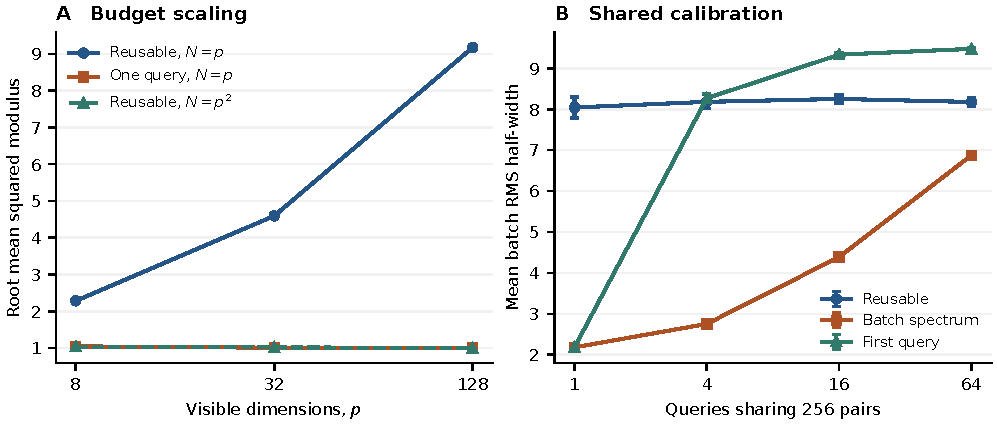
\includegraphics[width=.99\linewidth]{allocation.pdf}
\caption{Acquisition cost depends on which queries a common archive must serve. Panel A uses 512 Gaussian realizations per point. Panel B averages RMS half-width within each batch over 32 replicates at $p=64$. Bars show two Monte Carlo standard errors across independent batches. Each policy uses 256 pairs across the whole batch.}
\label{fig:allocation}
\end{figure}
At $N=p$, increasing $p$ from 8 to 128 increased the root mean squared modulus for balanced reusable acquisition from 2.28 to 9.17; the query-specific value stayed between 1.00 and 1.05. Spending $p^2$ pairs on reusable acquisition kept this modulus between 1.00 and 1.04. These values check the dimension dependence of Theorem~\ref{thm:budget}. For random batches of 16 queries in 64 dimensions with 256 shared pairs, the mean batch RMS half-width was 4.39 with the batch-spectrum design, 4.36 with mean-information allocation in that same basis, 8.25 with balanced reusable acquisition and 9.33 when all readings targeted the first query. The paired difference between reusable and batch-spectrum widths averaged 3.86 (Monte Carlo standard error 0.06). Across the 512 targets in that cell the corresponding empirical coverages were 96.5\%, 97.9\%, 98.4\% and 100\%, respectively. Learning which span must be served accounts for much of the width reduction.

We isolated the effect of allocating \emph{within} a known span in a supplemental comparison specified after the random-batch results. Each of 16 queries has norm 8 in 64 dimensions. With equal spectral energy the proposed and span-balanced schedules coincide. If one direction carries 75\% of batch energy and the other fifteen share the rest, the integer optimum assigns 76 of the 256 pairs to the leading direction. Compared with splitting the pairs equally within the same span, the integrated squared modulus falls from 4.224 to 2.067 and the RMS half-width from 4.48 to 3.44 across 256 fresh archives. The mean-information rule assigns 83 pairs to that direction, with squared modulus 2.076 and RMS half-width 3.44. The principal gain here comes from the anisotropy itself. Accounting for score-energy fluctuations makes a small difference to the allocation criterion.

\begin{table}[htbp]
\centering
\caption{Reusable archives on eight blur kernels. Columns show mean squared modulus $R^2$, mean of within-archive median half-widths $h_{50}$, and RMSE of the estimated conditional mean, averaged over archives and kernels. Each archive uses 64 held-out queries.}
\begin{tabular}{lrrrrrr}
\toprule
&\multicolumn{3}{c}{$N=32$}&\multicolumn{3}{c}{$N=256$}\\
\cmidrule(lr){2-4}\cmidrule(lr){5-7}
Allocation & $R^2$ & $h_{50}$ & RMSE & $R^2$ & $h_{50}$ & RMSE\\
\midrule
\inputrows camera_rows.tex
\bottomrule
\end{tabular}\label{tab:finitecamera}
\end{table}
The coupling in Table~\ref{tab:finitecamera} is held fixed across queries. It has norm 0.8 and equal squared loadings on the first direction and the uniform vector over the remaining coordinates. We used 16 archives per kernel and budget, and generated responses from the joint Gaussian law. At $N=256$, exact allocation reduces squared modulus from 38.00 for balanced acquisition to 20.07. Its median half-width falls from 8.59 to 7.87. At $N=32$ the ordering of actual widths reverses, despite the improvement in squared modulus. Focusing on four leading directions gives the best center RMSE for this particular coupling at both budgets. Coverage across all averaged policy-budget cells is at least 99.8\%. The table illustrates both the conservatism of the uniform half-width and the distinction between the allocation criterion and performance at one fixed population.

\subsection{Spatial holdouts with measured missing-band targets}
We used the corrected Indian Pines and Salinas AVIRIS cubes \cite{scenes}. We formed 24 visible variables by averaging successive groups of six among the first 144 retained bands. The target was the average of the last 16 retained bands at the same pixel. All pixel values and targets come from the published images. Each scene was split into four contiguous row strips. In each rotation, four disjoint strips supplied visible marginal moments, target-only moments, paired calibration objects and test targets respectively. Whitening used the visible strip alone; the target scale used the target-only strip. For deployment we added independent Gaussian noise with standard deviation 0.2 times the root mean visible-group variance. The calibration readings used the measured bands without added noise. We used every fourth test row and column, and 16 independent calibration samples at each budget. The archive for each method in a comparison contains the same pixels.

The eigenaxis designs project onto principal components of the visible-strip covariance. A band-group instrument instead reads a single one of the 24 visible groups on each paired pixel, cycling over the groups in a seeded order. In whitened coordinates its direction is the normalized loading vector of that band group. This comparator uses the same number of scalar readings and targets. Dense spectral projections and direct band readout can have different engineering costs. The study retrospectively computes both from full spectra.

\begin{table}[htbp]
\centering
\caption{Prediction of withheld measured bands. Each scene's numbers average equally over four held-out strips and 16 calibration samples per strip. Width is the mean of per-archive median half-widths. Width and RMSE use the target-only strip's standard deviation in each rotation. Coverage is empirical and reported in percent.}
\begin{tabular}{rlrrrrrr}
\toprule
& &\multicolumn{3}{c}{Indian Pines}&\multicolumn{3}{c}{Salinas}\\
\cmidrule(lr){3-5}\cmidrule(lr){6-8}
$N$&Allocation&Width&Coverage&RMSE&Width&Coverage&RMSE\\
\midrule
\inputrows scene_rows.tex
\bottomrule
\end{tabular}\label{tab:scenes}
\end{table}

For Indian Pines at 256 pairs, the exact allocation gives mean median half-width 2.34 and mean coverage 97.0\%. Its four strip coverages average 95.8--97.9\% individually over the 16 archives. Direct band groups require half-width 3.68 and cover 99.6\%. The mean-information rule gives 2.33 and 96.3\%; proportional allocation gives 2.34 and 96.5\%. Similar width for these spectral allocations limits the evidence for an advantage from the exact integer marginal returns on this scene. The marginal-only interval, centered on the separate target strip with half-width 1.96, covers 87.9\% overall, ranging from 60.1\% to 100\% across strips.

Salinas shows a substantial failure of spatial transfer. At 256 pairs the exact allocation has half-width 2.03 and empirical coverage 56.8\%. The four strip coverages are 45.8\%, 58.2\%, 97.8\% and 25.5\%. The direct band-group archive covers 70.9\% at half-width 2.59, and the target-only interval covers 45.9\%. Raising the budget from 32 to 256 narrows the exact-allocation interval from 2.50 to 2.03 while its center RMSE stays at 2.04 and coverage falls from 76.1\% to 56.8\%. More paired pixels from one strip do not ensure calibration on another. Each scene provides four spatial holdouts; the 16 archives per rotation resample calibration pixels and deployment noise around the same held-out targets. Treating them as independent scenes would understate spatial uncertainty.

We examined target marginals after seeing the coverage results. In the worst Salinas fold the held-out target mean is 2.28 target-reference standard deviations above the reference-strip mean, and its standard deviation is 1.22 times the reference value. Across the four Indian Pines folds the absolute mean shifts range from 0.41 to 1.35 standard deviations. These diagnostics document a violation of the common-marginal assumption. They do not by themselves distinguish the contributions of changing marginals, conditional structure and non-Gaussianity to the coverage errors.
